\documentclass[11pt]{paper}
\title{An introduction to Migen}
\subtitle{Version: February 7th 2014}
\author{S\'ebastien Bourdeauducq}
\usepackage{palatino}
\usepackage{color}
\usepackage{fullpage}
\usepackage{url}
\usepackage{tabularx}
\usepackage{graphicx}
\usepackage{moreverb}
\usepackage[utf8]{inputenc}
\definecolor{mygray}{gray}{0.92}
\setlength{\parindent}{0in}
\setlength{\parskip}{8pt}
\begin{document}

\newcommand{\mybox}[1] {\fcolorbox{black}{mygray}{\parbox{\textwidth}{#1}}\hspace{2pt}}

\maketitle

\textit{This tutorial gives a first introduction to FPGA design using Migen. It assumes some knowledge of Unix commands, Python programming language and logic design.}

\section{Software setup}
\subsection{Third-party tools}
This tutorial requires a Linux machine with Python 3.3+, Git and Xilinx ISE. Note that Migen cannot be used with Python 2, but most Linux distributions allow you to easily install both Python 2 and Python 3 on the same machine.

\subsection{Migen}
We simply obtain the sources from the Git repository and set the \verb!PYTHONPATH! environment variable so that Python searches that directory when importing modules.

Alternatively, Migen can be permanently installed on your system by running its \verb!setuptools! script (\verb!python3 setup.py install!)

\begin{verbatim}
$ git clone git://github.com/m-labs/migen.git
$ export PYTHONPATH=`pwd`/migen
\end{verbatim}

\subsection{Simulator}
\textit{This step can be skipped if you do not intend to use the simulator.}

Migen relies on an external Verilog simulator to simulate your designs. It is known to work with Icarus Verilog.

\mybox{Make sure that your installed version of Icarus Verilog is recent enough to include commit b85e7efca86757c4a752bbba5de2127fe9df0a13 (from April 2, 2012). The bug that this commit fixes makes the Migen simulator completely dysfunctional.}

To communicate with Icarus Verilog, the Migen simulator uses a UNIX domain socket and a custom protocol which is handled by a VPI plug-in (written in C) on the Icarus side.

To build and install this plug-in, run the following commands from the \verb!vpi! directory in the Migen source tree:

\begin{verbatim}
$ make [INCDIRS=-I/usr/...]
$ make install [INSTDIR=/usr/...]
\end{verbatim}

The variable \verb!INCDIRS! (default: empty) can be used to give a list of paths where to search for the include files. This is useful considering that different Linux distributions put the \verb!vpi_user.h! file (shipped with Icarus Verilog) in various locations.

The variable \verb!INSTDIR! (default: \verb!/usr/lib/ivl!) specifies where the \verb!migensim.vpi! file is to be installed.

A VCD file viewer such as GTKWave should also be installed.

\section{First steps}
A central component of Migen is the FHDL layer. It allows you to create and manipulate logic designs in Python and convert them to synthesizable Verilog.

Run a Python interpreter and import the Migen FHDL declarations:
\begin{verbatim}
$ python3
>>> from migen.fhdl.std import *
\end{verbatim}

The basic building block of a FHDL design is the \verb!Signal! object. It serves the same purpose as \verb!signal! in VHDL and \verb!wire! or \verb!reg! in Verilog.

We create two such signals, having a width of 1 bit each:
\begin{verbatim}
>>> a = Signal(1)
>>> b = Signal(1)
\end{verbatim}

\mybox{The width of 1 is the default, so one can also simply write Signal().}

We would now like to represent Boolean equations between signals, for example the \verb!OR! of these two signals we just created. Migen provides the \verb!_Operator! object for this purpose, but since using it directly results in a very cluttered syntax, it also redefines the basic Python operations on signals so that such \verb!_Operator! objects can be created in a much lighter way:

\begin{verbatim}
>>> a | b
<migen.fhdl.structure._Operator object at 0x965e14c>
\end{verbatim}

Let's examine the contents of our newly-created object:
\begin{verbatim}
>>> tmp = a | b
>>> tmp
<migen.fhdl.structure._Operator object at 0x965e86c>
>>> tmp.op
'|'
>>> tmp.operands
[<Signal a at 0xb6f7ae2c>, <Signal b at 0x965e82c>]
\end{verbatim}

As you can see, the object contains the information to represent our \verb!OR! gate. \verb!_Operator! objects can be of course combined to form expression trees (of arbitrary complexity):
\begin{verbatimtab}
>>> c = Signal()
>>> tmp = a | (b & c)
>>> tmp
<migen.fhdl.structure._Operator object at 0x965eeac>
>>> tmp.op
'|'
>>> tmp.operands
[<Signal a at 0xb6f7ae2c>, 
  <migen.fhdl.structure._Operator object at 0x965e56c>]
>>> tmp.operands[1].op
'&'
>>> tmp.operands[1].operands
[<Signal b at 0x965e82c>, <Signal c at 0xb6f6c0ec>]
\end{verbatimtab}

We now have a means of representing Boolean equations involving signals. We would now like to assign such expressions to other signals. FHDL provides the \verb!_Assign! object for this purpose, as well as a technique to create it easily using the \verb!eq! method of \verb!Signal! objects:
\begin{verbatim}
>>> x = Signal()
>>> tmp = x.eq(a | b)
>>> tmp
<migen.fhdl.structure._Assign object at 0xa2371ec>
>>> tmp.l # left hand-side of assignment
<Signal x at 0xa23756c>
>>> tmp.r # right hand-side of assignment
<migen.fhdl.structure._Operator object at 0xa23790c>
\end{verbatim}

In a typical FPGA design, an assignment can be triggered by two types of events:
\begin{enumerate}
\item whenever an input changes \textit{(combinatorial assignment)}
\item at the edge of the clock signal \textit{(synchronous assignment)}
\end{enumerate}

Defining when an assignment takes place is done by using the in-place addition operation (\verb!+=!) on special properties of a \verb!Module! object. The \verb!comb! special property makes the assignment combinatorial, while the \verb!sync! property synchronizes it with the default (aka system) clock.

\mybox{Migen supports designs with multiple clock domains, but they are beyond the scope of this tutorial.}

We can now fully model a pure (combinatorial) \verb!OR! gate between signals \verb!a!, \verb!b! and \verb!x!:
\begin{verbatim}
>>> my_or = Module()
>>> my_or.comb += x.eq(a | b)
\end{verbatim}

Modules are convertible to Verilog. Note the \verb!ios! option of the \verb!convert! function, that specifies which signals (in our case, all of them) should be exported as inputs/outputs of the Verilog module. Without that option, signals would stay inside the Verilog module (try it).
\begin{verbatimtab}
>>> from migen.fhdl import verilog
>>> print(verilog.convert(my_or, ios={a, b, x}))
/* Machine-generated using Migen */
module top(
        input a,
        input b,
        output x
);


// synthesis translate off
reg dummy_s;
initial dummy_s <= 1'd0;
// synthesis translate on
assign x = (a | b);

endmodule
\end{verbatimtab}

\section{A LED blinker}
\subsection{Design}
We are now ready for a slightly more complicated design. It consists of a decrementing counter, which, when it reaches 0, toggles a one-bit signal (which will blink a LED) and reloads from another signal (that controls the period of the toggling).

Create a file \verb!ledblinker.py! containing the following:

\begin{verbatimtab}
from migen.fhdl.std import *
from migen.fhdl import verilog

class Blinker(Module):
	def __init__(self, led, maxperiod):
		counter = Signal(max=maxperiod+1)
		period = Signal(max=maxperiod+1)
		self.comb += period.eq(maxperiod)
		self.sync += If(counter == 0,
				led.eq(~led),
				counter.eq(period)
			).Else(
				counter.eq(counter - 1)
			)

led = Signal()
my_blinker = Blinker(led, 30000000)
print(verilog.convert(my_blinker, ios={led}))
\end{verbatimtab}

Take note of the following points:
\begin{itemize}
\item we are inheriting from the \verb!Module! class. This is the preferred way of creating a component in Migen, rather than instantiating \verb!Module! directly and externally using its special properties as we did before. In a more complex design, a module can integrate other modules by using the \verb!submodules! special property.
\item another way to create multi-bit signals is to use the \verb!max! parameter of the constructor, which specifies the exclusive upper bound that the value of the signal can reach. There is a similar \verb!min! parameter. Both \verb!min! and/or \verb!max! can be negative, in which case Migen will use two's complement arithemetic to represent negative values.
\item we use the \verb!If! object, which represents conditional statements (which have the same sense as in Verilog or VHDL). Another Python syntax trick is used here for \verb!Else!, which is actually a method of the \verb!If! object that modifies the latter when called and inserts the statement list for the ``false'' part of the conditional.
\end{itemize}

Run this script and examine the generated Verilog source.

\mybox{As an exercise, you can add a control signal that toggles between a high and a slow blinking frequency. Conditional statements can also be used in combinatorial lists (as in Verilog or VHDL). When using += on a special Module property, the statement(s) you specify are added to the existing statements in that module.}

\subsection{Simulation}
For the purposes of the simulation, set the period signal to a lower value, e.g. 5. Add the following to the script:
\begin{verbatimtab}
from migen.sim.generic import run_simulation

...

run_simulation(my_blinker, ncycles=200, vcd_name="ledblinker.vcd")
\end{verbatimtab}

You can remove the import of the \verb!migen.fhdl.verilog! module and the printing of the Verilog source. Running the script now produces a VCD file which you can open with GTKWave:
\begin{verbatim}
$ gtkwave ledblinker.vcd
\end{verbatim}

\begin{figure}[h]
\centering
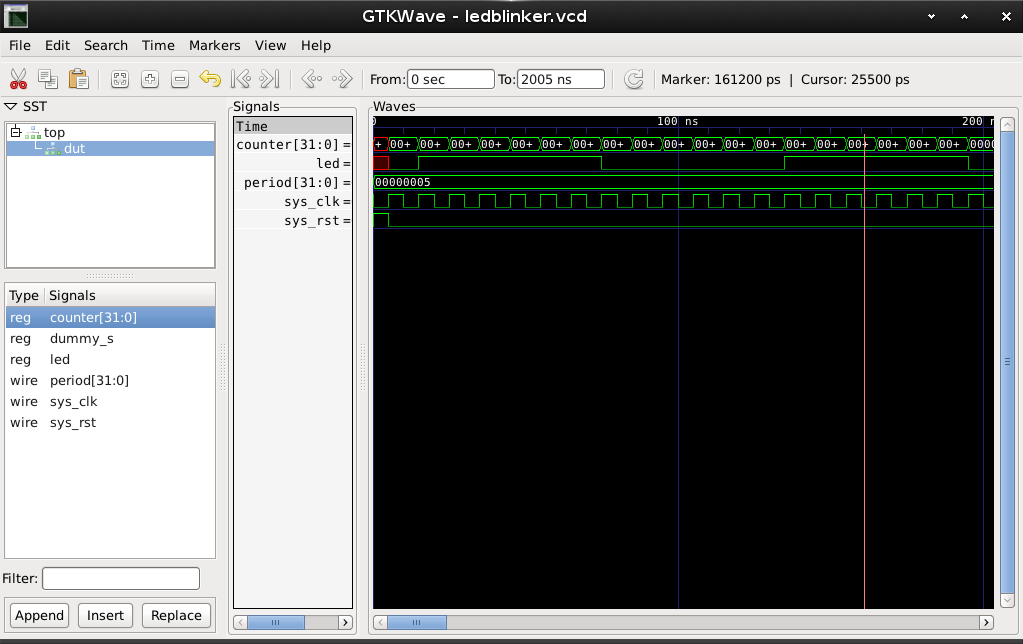
\includegraphics[width=\textwidth]{gtkwave.png}
\caption{LED blinker signals in GTKWave.}
\end{figure}

Notice that a clock and reset signal have been added automatically.

Since observing waveforms manually is a tedious and error-prone process, Migen lets you read and write simulated signals from Python. All the libraries and features that Python offers can be used, which enables you to create powerful test benches. In this tutorial, we will simply print out at which clock cycles the transitions on \verb!led! occur.

Add the following code to the script:
\begin{samepage}
\begin{verbatimtab}
...
class Blinker(Module):
	def __init__(self, led, maxperiod):
		self.led = led
		self.v_led_old = 0
		...

	def do_simulation(self, selfp):
		v_led = selfp.led # read the current signal value
		if v_led != self.v_led_old:
			print("{old}->{new} cycle={cycle}".format(
				old=self.v_led_old, new=v_led,
				cycle=s.cycle_counter))
			self.v_led_old = v_led
\end{verbatimtab}
\end{samepage}

We are using another \verb!Module! feature, the \verb!do_simulation! method. At each simulated clock cycle, the Migen simulator runs this function in each \verb!Module!, passing it a ``proxy'' object in the \verb!selfp! parameter that mirrors the module and lets the function manipulate the values of the signals. Reading a proxy attribute corresponding to a signal from the module returns the value of the signal, and writing to the proxy attribute sets the value of the signal.

Run the simulator again. It should run the \verb!do_simulation! method and produce the following output:
\begin{verbatimtab}
0->1 cycle=1
1->0 cycle=7
0->1 cycle=13
1->0 cycle=19
0->1 cycle=25
1->0 cycle=31
0->1 cycle=37
1->0 cycle=43
...
\end{verbatimtab}

\mybox{As an exercise, you can add code that verifies that the transitions are happening on the intended edges (i.e. make the test bench self-checking).}

\subsection{Hardware implementation}
Revert any code changes you have done for simulation purposes and go back to the original design (you can still leave out the explicit conversion to Verilog).

Hardware implementation on supported boards is greatly simplified by using the Mibuild library which is distributed with Migen. This tutorial assumes you have a Mixxeo, a Milkymist One, a Papilio Pro or a RHINO board. Import the corresponding module with one of the following lines:

\begin{verbatimtab}
from mibuild.platforms import mixxeo as board
from mibuild.platforms import m1 as board
from mibuild.platforms import papilio_pro as board
from mibuild.platforms import rhino as board
\end{verbatimtab}

\mybox{See the ``platforms'' folder in the Mibuild sources for a complete list of supported boards. You can also add your own and submit it for inclusion into Mibuild. Altera boards are also supported.}

Next, create a platform object and obtain the \verb!led! signal from Mibuild instead of creating it yourself:
\begin{verbatimtab}
plat = board.Platform()
led = plat.request("user_led")
my_blinker = Blinker(led, 30000000)
\end{verbatimtab}

You are now ready to build the bitstream! Mibuild will add a default clock, which has a frequency of 50MHz on the Mixxeo and Milkymist One, 32MHz on the Papilio Pro and 100MHz on the RHINO.
\begin{verbatimtab}
plat.build_cmdline(my_blinker)
\end{verbatimtab}

Run the script with those modifications, and after a too long compilation process, you will obtain a \verb!top.bit! bitstream file in a newly created folder \verb!build!.

Mibuild assumes the Xilinx tools are installed in \verb!/opt/Xilinx!. If they are not, run your script as follows: \verb!python3 ledblinker.py --ise-path /path_to_ise!

Load the bitstream file using the appropriate programming tool for your board, and you should see the LED blinking. The Mixxeo, Milkymist One and Papilio Pro boards can be programmed with UrJTAG:

\begin{verbatim}
$ jtag
jtag> cable milkymist # for Mixxeo and Milkymist One
jtag> cable Flyswatter # for Papilio Pro
jtag> detect
jtag> pld load build/top.bit
\end{verbatim}

\section{To go further}
This tutorial has given you an overview of the base component of Migen, FHDL. It enables developers to use the full power of Python to generate and verify the logic of their designs.

Migen comes with many other components and features that use FHDL to build system-on-chip interconnect, dataflow systems, configuration and status register banks, finite state machines, and more. Read the Migen manual available at \url{http://m-labs.hk/gateware.html} for a more complete description. A heavy user of Migen is the MiSoC system-on-chip, whose source code you can obtain from the same webpage.

Direct questions and feedback about Migen or this tutorial to the devel@lists.m-labs.hk mailing list or the IRC channel \#m-labs on Freenode.

\end{document}
